\newpage
\section{Auswertung}
\subsection{Effektiver Dämpfungswiderstand und Abklingdauer}
Anhand der zeitabhängigkeit der Amplitude wird der Effektive Dämpfungswiderstand $R_{eff}$
und die Abklingdauer $T$ bestimmt. 
\begin{figure}
    \centering
    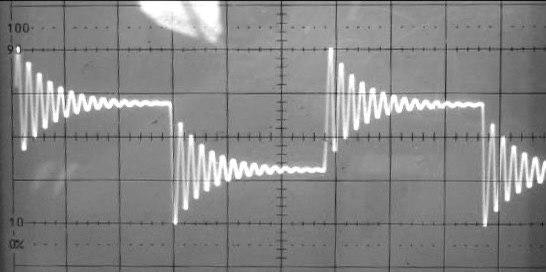
\includegraphics[width=0.7\textwidth]{bilder/Bild_5a_screen.jpg}
    \caption{
        Gemessene Kondensatorspannung bei einem RCL-Kreis mit angelegter Rechteckspannung. 
        Mit t $20\mu s/Div.$ und V $ 2V/Div.$
        }
    \label{fig:bild1}
\end{figure}

\begin{table}
    \centering
    \begin{tabular}{c c}
        \toprule
        $U(t)\;/\;2V$ & $t\;/\;20\mu s$\\
        \midrule
        2,0     &0   \\
        1,6     &0,25\\
        1,4     &0,45\\
        1,25    &0,6\\
        1,1     &0,9\\
        1,05    &1,0\\
        1,0     &1,2\\
        0,9     &1,4\\
        0,8     &1,6\\
        0,7     &2,7\\
        \bottomrule
    \end{tabular}
    \caption{Amplituden aus gedämpften Schwingkries gegenüber der Zeit}
    \label{tab:tabelle1}
\end{table}

Mit dem Widerstand $R1=(30.3\pm0.01)\si{\ohm}$, der Induktivität $L=(3.5 \pm 0.01)mH$ der Schaltung und $y_0=2.6V$ folgt die Theoriekurve
\begin{align}
    y(t)&=2.6 \cdot e^{-R/2L \cdot t}\\
    y(t)&\approx 2.6 \cdot e^{-(4,33\pm0,01) \cdot 10^3*t}
\end{align}
\newpage
Insgesamt ergibt sich somit für die Messdaten und dessen Ausgleichsfunktion $y(t)=e^{-k*t}$
sowie für die Theoriekurve:
\begin{figure}
    \centering
    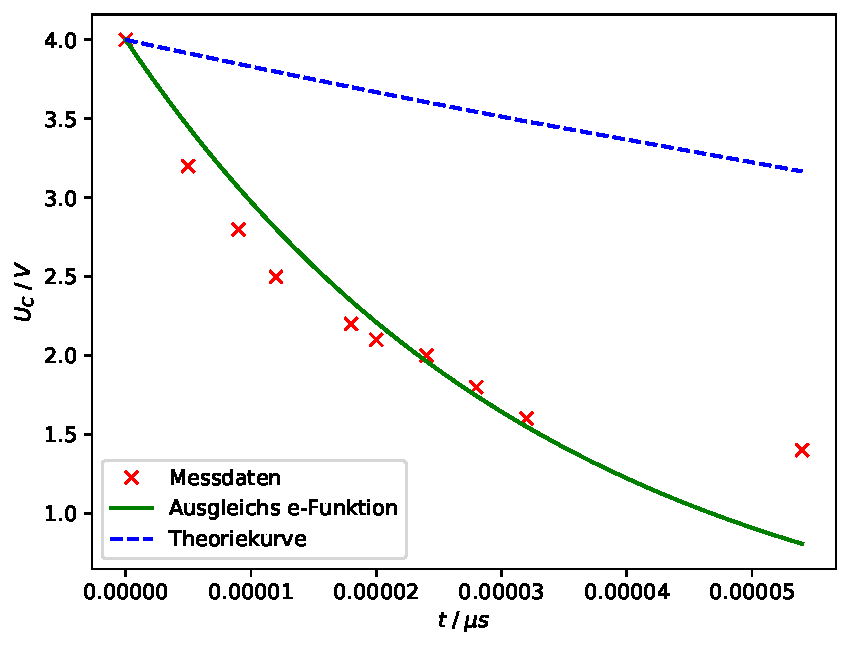
\includegraphics[width=0.7\textwidth]{bilder/plota.pdf}
    \caption{
        Darstellung der Daten der einhüllenden der gedämpften Schwingungen mit ihrer
        Ausgleichsfunktion $y(t)\approx 4 \cdot e^{-6,82\cdot10^4 \cdot t}$ verglichen mit der Theoriekurve
    }
    \label{fig:ultra_plot}
\end{figure}



Aus den Daten und der Ausgleichsfunktion folgt somit der effektive Dämpfungswiderstand 
$R_{eff}$
\begin{equation}
    R_{eff}= (4,77 \pm 0,12)\cdot10^3 \cdot 2L \approx (33,34 \pm 0,84) \si{\ohm}
\end{equation}
Die Abklingdauer $T_{ex}$ ergibt sich somit
\begin{equation}
    T_{ex}=\frac{2L}{R_{eff}}\approx 1,47 \pm 0,04) \cdot 10^{-5}s
\end{equation}






\subsection{Aperiodischer Grenzfall}
Der Spezialfall liefert:
\begin{equation}
    R_{ap}^{Theorie}=\sqrt{\frac{4L}{C}}=1673,32\si{\ohm}     %fehler und Fehlerrechnung fehlt
\end{equation}
Durch regelbaren Widerstand und das vermeiden eines Überschwingens ergibt sich
\begin{equation}
    R_{ap}^{Exp}=1475\si{\ohm}
\end{equation}
\begin{figure}
    \centering
    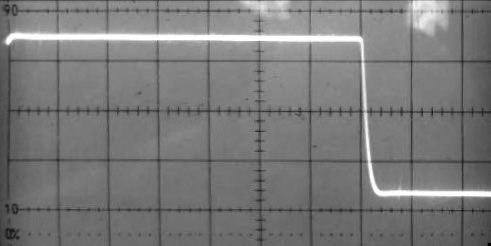
\includegraphics[width=0.5\textwidth]{bilder/Aperiodischer_grenzfall_screen.jpg}
    \caption{Der aperiodische Grenzfall mit einem Regelbaren Widerstand. Dieser ist so justiert, das gerade eben kein Überschwingen eintritt.}    %Oszilloskop daten hinzufügen Div.
\end{figure} 
\newpage







\subsection{Kondensatorspannung und ihre Frequenzabhängigkeit}
\begin{table}
    \centering
    \begin{tabular}{c c}
        \toprule
        $w\;/\;kHz$ & $U_C(t)\;/\;V$\\
        \midrule
        28      &3,2\\
        29      &3,4\\
        30      &3,6\\
        31      &3,7\\
        32      &3,9\\
        33      &4,0\\
        34      &4,2\\
        35      &4,4\\
        36      &4,4\\
        37      &4,3\\
        38      &4,1\\
        39      &4,0\\
        40      &3,8\\
        41      &3,6\\
        42      &3,2\\
        \bottomrule
    \end{tabular}
    \caption{Kondensatorspannung $U_C$ in Abhängigkeit der Frequenz}
    \label{tab:tabelle_w}
\end{table}
\begin{figure}[H]
    \centering
    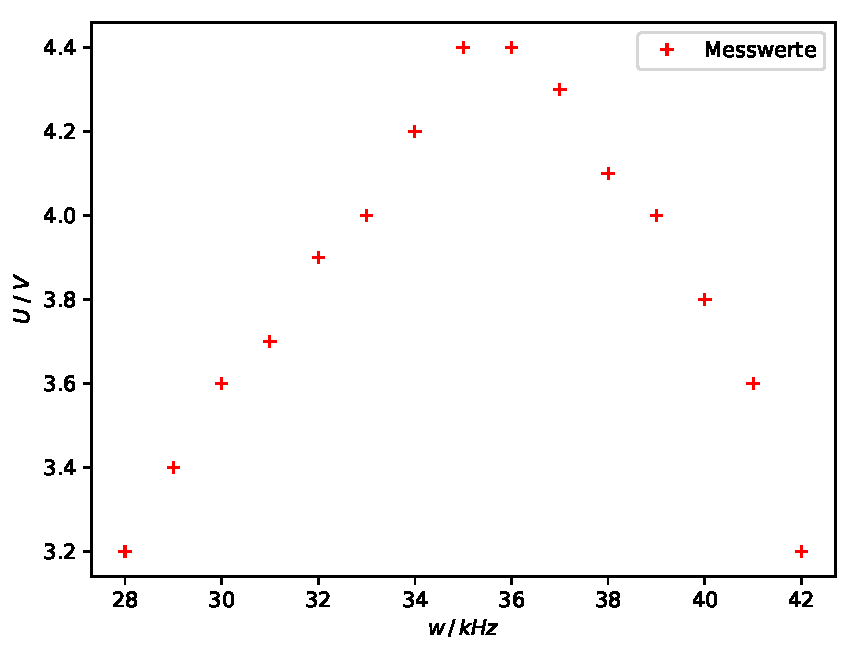
\includegraphics[width=0.5\textwidth]{bilder/plotc.pdf}
    \caption{
        Daten aus \ref{tab:tabelle_w} in Abhängigkeit von der Kondensatorspannung $U_C$ dargestellt
    }
\end{figure}
Grund für die Frequenzabhängigkeit sind die komplexen Widerstände von Spule und Kondensator.
Der Betrag der Impedanz ergibt sich dabei aus
\begin{equation}
    |Z_{ges}|=\sqrt{R^2+(\omega L-\frac{1}{\omega C})^2}
\end{equation}
mit den Schwingkreis Komponenten $R=(271,6\pm0,2)\si{\ohm}$, $L=(3,5\pm 0,01)10^(-3)H$ und $C=(5,00\pm 0,2)10^(-90F)$ ergibt 
sich die Impedanzkurve
\begin{figure}[H]
    \centering
    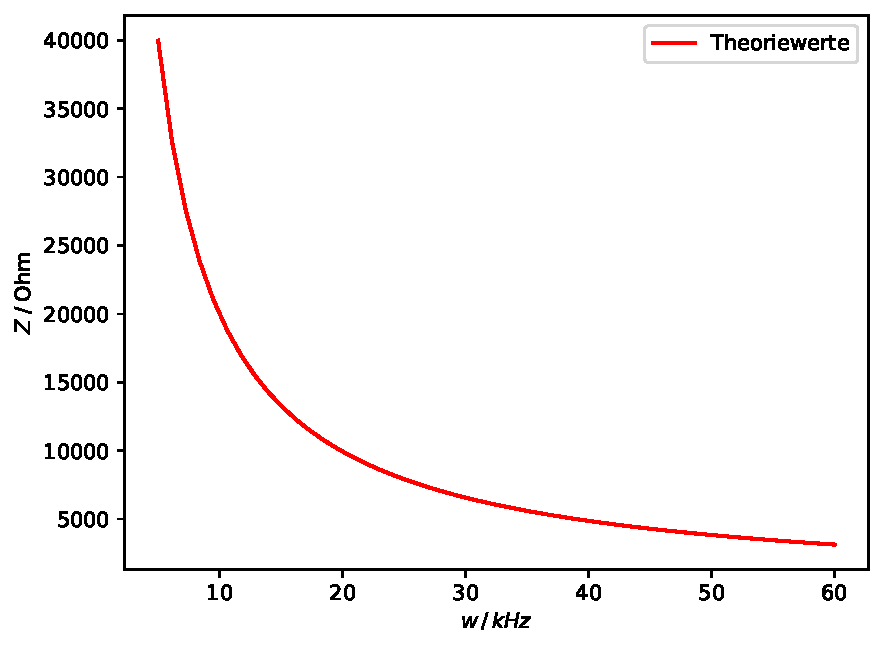
\includegraphics[width=0.5\textwidth]{bilder/plotZ.pdf}
    \caption{
        Frequenzabhängige Widerstände. Die Spannung ist proportional zur Impedanz $Z$
    }
    \label{fig:Frequenzabh_Wiederstand}
\end{figure}
\newpage





\subsection{Phasenverschiebung}
Nach der Methode in Abbildung \ref{eqn:phase} kann nun die Phasenverschiebung $\phi$
zwischen Erreger- und Kondensatorspannung bestimmt werden. 
\begin{table}
    \centering
    \begin{tabular}{c c c c}
        \toprule
        $w\;/\;kHz$ & $a$ & $b$ & $\Delta \phi\;/\;$rad\\
        \midrule
        42,0 & 1,6 & 4,2 & 1,2 \\
        41,0 & 1,5 & 4,4 & 1,07 \\
        40,0 & 1,4 & 4,5 & 0,98 \\
        39,0 & 1,4 & 4,6 & 0,96 \\
        38,0 & 1,3 & 4,7 & 0,87 \\
        37,0 & 1,2 & 4,8 & 0,79 \\
        36,0 & 1,1 & 5,0 & 0,69 \\
        35,0 & 1,0 & 5,1 & 0,62 \\
        34,0 & 0,8 & 5,3 & 0,47 \\
        33,0 & 0,8 & 5,5 & 0,46 \\
        32,0 & 0,8 & 5,6 & 0,45 \\
        31,0 & 0,8 & 5,8 & 0,43 \\
        30,0 & 0,7 & 5,8 & 0,38 \\
        29,0 & 0,6 & 6,0 & 0,31 \\
        \bottomrule
    \end{tabular}
    \caption{Die Phasenverschiebung $\Delta \phi$ zwischen der sinusförmigen Erregerspannung $\tilde{U}(t)$ und der Kondensatorspannung $U_C(t)$}
    \label{tab:tabelle_phi}
\end{table}
\begin{figure}
    \centering
    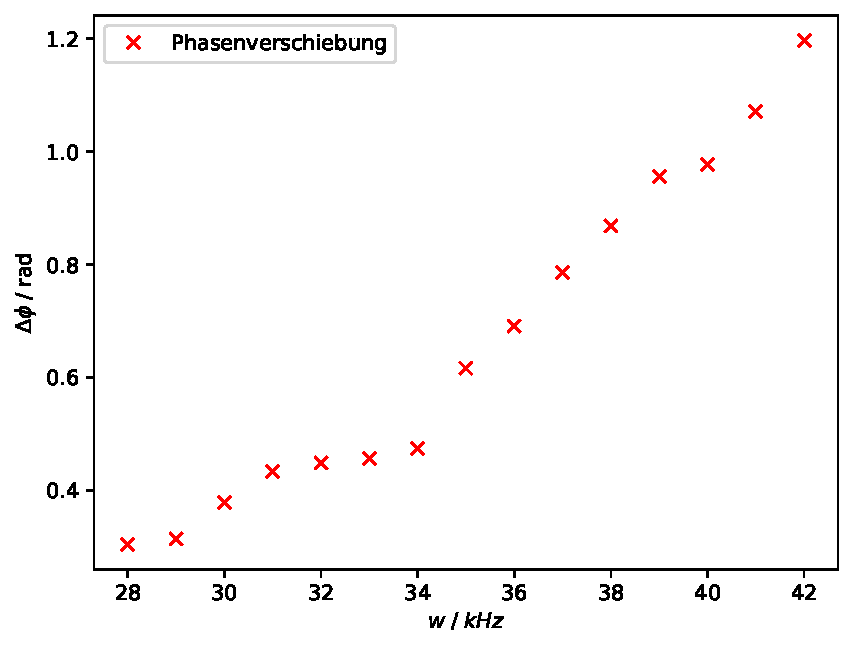
\includegraphics[width=0.5\textwidth]{bilder/plotph.pdf}
    \caption{
        Berechnete Werte für die Phasenverschiebung $\Delta \phi$ aus \ref{tab:tabelle_phi} 
    }
\end{figure}





\label{sec:Auswertung}